% This is samplepaper.tex, a sample chapter demonstrating the
% LLNCS macro package for Springer Computer Science proceedings;
% Version 2.20 of 2017/10/04
%
\documentclass[runningheads]{llncs}
%
\usepackage[utf8]{inputenc}
\usepackage{listings}
\usepackage{xcolor}
\usepackage{graphicx}
\usepackage{tabularx}
\usepackage{hyperref}

\graphicspath{ {./images/} }
\hypersetup{
    colorlinks=true,
    linkcolor=blue,
    filecolor=blue,
    citecolor=blue,
    urlcolor=blue,
    linktocpage=true
}
\setcounter{tocdepth}{2} %show more in the toc

\newcommand{\kw}[1]{\texttt{#1}}
\renewcommand{\contentsname}{table of content}
\usepackage{indentfirst}
\usepackage[english]{babel}

% If you use the hyperref package, please uncomment the following line
% to display URLs in blue roman font according to Springer's eBook style:
\renewcommand\UrlFont{\color{blue}\rmfamily}

%

\title{Infra-estrutura de Testes para Implementações de Referência do Standard ECMAScript}
\subtitle{}

%
\titlerunning{Live Metadata for Test262}
% If the paper title is too long for the running head, you can set
% an abbreviated paper title here
%
\author{Diogo Costa Reis\\ist187526\\
\email{diogo.costa.reis@tecnico.ulisboa.pt}}
%
\authorrunning{Diogo Costa Reis}
% First names are abbreviated in the running head.
% If there are more than two authors, 'et al.' is used.
%
\institute{Instituto Superior Técnico\\
Av. Rovisco Pais, 1\\
1049-001 Lisboa\\
Tel: +351 218 417 000\\
\email{mail@tecnico.ulisboa.pt}}
%


\begin{document}

% a solution to remove title and author from appearing in the table of contents: https://tex.stackexchange.com/a/318220
{\def\addcontentsline#1#2#3{}\maketitle}

%
\begin{abstract}
% TODO

\keywords{ECMAScript \and Specification Language \and Reference Interpreters \and Test262}
\end{abstract}


\newpage

\tableofcontents

\newpage

\section{Introduction}
\label{sec:Introduction}

\section{Goals}
\label{sec:Goals}

\section{Background}
\label{sec:Background}
This chapter provides an overview on the ECMAScript standard, the Test262 that are used to test the correct implementation of the ECMAScript standard, and finally an outline of the new metadata generated.

\subsection{ECMAScript}
\label{subsec:ECMAScript}
% overview da linguagem JS

% paragrafo - porque e' que javascript e' relevante (uma das linguagens mais usadas no momento)
JavaScript (JS) is a programming language mainly used in the development of client side web applications, also being one of the most popular programming languages. According to both GitHub and StakeOverflow statistics, JavaScript finished 2021 as second most active languages on GitHub\footnote{Second most utilized language based GitHub pull requests - https://madnight.github.io/githut/} as well as on StackOverflow.\footnote{Tendencies based on the Tags used - https://insights.stackoverflow.com/trends}



% Boa!
% Existem muitas implementacoes diferentes da linguagem: client-side (browsers), server-side (Node.js), embedded devices (Jerryscript) -> Estas implementacoes têm de estar de acordo no comportamento observavel -> é particularmente importante na Web -> senao temos sites que em ...
% -----------------------
% overview do standard -> descrita num standard
% Porque é muito importante que as várias implementacoes da linguagem coincidam -> o JavaScript está especificado num documento semi-formal que ...
% Falar sobre o standard
%   - o standard está como um interpretador de JavaScript em
%     pseudo-codigo - descreve detalhadamente os passos que
%    um interpretador de JS tem de executar ao avaliar qualquer
%    statement da linguagem
% Falar sobre o comité -  quem controla a evolucao do ECMAScript
ECMAScript standard\cite{ECMAScriptStandard} is the official document, written in the English language, in which the JavaScript language is defined. This document is in constant evolution, being updated by the ECMA Technical Committee 39 (TC39), which is responsible for maintaining the standard. The standard is currently in its twelfth version.
%
The standard specifies the \texttt{JavaScript} language, to ensure its multiple compilers and interpreters implementations are coherent. Some of the \texttt{JavaScript} compilers are the Hop~\cite{Hop} and the JSC~\cite{JSC} compilers, the most popular interpreters are Node.js~\cite{Node.js} and SpiderMonkey~\cite{SpiderMonkey}. These are only four implementations among many others, which come along with the many use cases that \texttt{JavaScript} has.
%
\texttt{JavaScript} is mostly used in the web context, both client-side within browsers and server-side, but also in embedded devices. Since \texttt{JavaScript} is used in so many scenarios and across so many different contexts, it is highly important that ECMAScript standard is defined in great detail to ensure consistency. Browsers, for example, need to run \texttt{JavaScript} implementations that coincide so that websites are correctly rendered and exhibit the same behavior. In order to achieve coherent implementations, the standard defines the types, values, objects, properties, syntax, and semantics of \texttt{JavaScript} that must be the same in every \texttt{JavaScript} compiler and interpreter, while allowing \texttt{JavaScript} implementations to define additional types, values, object, properties, and functions.




% Good, more detail if there is time
% Estrutura do standard
The \texttt{JavaScript} language can be divided into three major components, those being expressions and commands, built-in libraries, and finally internal functions.
%
\begin{itemize}
\item Expressions and commands describe the behavior of static constructions, detailing the semantics of the diverse expressions (e.g., assignment expressions, built-in operators, etc.), commands (e.g., loop commands, conditions command, etc.), and built-in types (Undefined, Null, Boolean, Number, String and Object).
%
\item The internal functions of the language are used to define the semantics for both expressions and commands, as well as the built-in libraries. Internal functions are not exposed beyond the internal context of the language. In other words, no JavaScript program uses internal functions directly.
%
\item Finally, built-in libraries encompass all the internal objects available when a JavaScript program is executed. Internal objects expose many functions implemented by the language itself, including functions to manipulate numbers, text, arrays, objects, among other things.
\end{itemize}


% MetaParagrafo tres tipos
\colorbox{orange}{The remaining} subsection provides a description of the three types of artifact described in the standard.
% QUESTION ainda nao foi lido pelo prof

% Expressions and statements
% Exemplo do standard  e explicacao (if)
\paragraph{Semantics of IF statement}
Figure \ref{fig:If-Else Statement} shows a snippet of the ECMAScript standard description of the \texttt{IF} command. In order to evaluate \texttt{IF} commands with the shape:

\begin{center}
\texttt{if (Expression) Statement1 else Statement2}
\end{center}

\noindent the language begins by evaluating the \texttt{Expression} storing the result in the variable \texttt{exprRef} (step 1). The previous step will be used as Boolean, therefore, the result of the previous step will be converted to a Boolean using the internal functions \texttt{ToBoolean} and \texttt{GetValue}, and having the result stored in the variable \texttt{exprValue} (step 2).A different \texttt{Statement} will be followed depending on \texttt{exprValue}. If \texttt{exprValue} has the value \texttt{true} the variable \texttt{stmtCompletion} will have the evaluation of the first \texttt{Statement} (step 3). Otherwise, the variable \texttt{stmtCompletion} will store the result of evaluating the second \texttt{Statement} (step 4). Finally, a \texttt{Completion} will be returned, if the \texttt{stmtCompletion} has non empty value then it will be returned, however, when the value is empty it will be replaced with undefined (step 5).

\begin{figure}[ht]
    \centering
    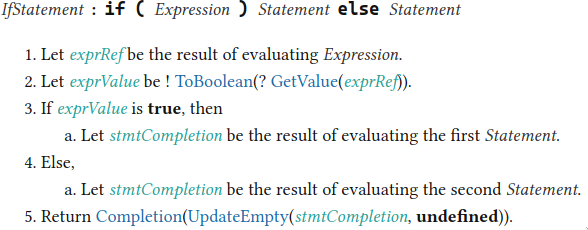
\includegraphics[width=0.8\textwidth]{images/if_statement.png}
    \caption{ECMAScript definition of an if-else statement}
    \label{fig:If-Else Statement}
\end{figure}

% arrays são objetos como os outros
% arrys tem propriedades especiais
% example of Array.pop
% Built-ins (Array.pop)
% printscreen do standard e explicacao
\paragraph{Semantics of the Pop function}
The Array built-in is an object as any other in JavaScript. The main difference is in its properties. Array Objects have a property \texttt{length} that contains the size of the array, as well as a property for each element of the array (from zero to \texttt{length} minus 1).

Figure \ref{fig:Array_pop_example} shows a simplified version of an array performing the pop function, where \texttt{(a)} and \texttt{(b)} are the before and after respectively.
Before preforming \texttt{pop} \texttt{(a)}, the array has three  properties \texttt{length}, \texttt{0}, and \texttt{1}. Property \texttt{length} represents the size of the array that has value \texttt{2}, while the properties \texttt{0} and \texttt{1} store the first (\texttt{banana}) and second (\texttt{kiwi}) elements of the array respectively.
After \texttt{pop} is preformed \texttt{(b)}, the last element is of the array is removed (highlighted in red at \texttt{(a)}) and the \texttt{length} property (highlighted in green) is decremented by one since the size of the array changes to one.

% TODO change length with quotation marks
\begin{figure}[ht]
    \centering
    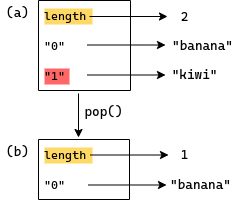
\includegraphics[width=0.4\textwidth]{images/array_pop_example.png}
    \caption{Example Array.pop}
    \label{fig:Array_pop_example}
\end{figure}
Figure \ref{fig:Array_pop} shows a snippet of the ECMAScript standard description of the pop function in the Array Built-in. To begin with, the array will be converted to and Object using the \texttt{ToObject} function, and stored in the \texttt{O} variable (step 1).
Afterwards, the array length of the previously calculated variable will be calculated with the \texttt{LengthOfArrayLike} internal function, and storing the result in the \texttt{len} variable (step 2).
At this point there are to ways to proceed depending on the value of \texttt{len}. If the value is zero, the Array is empty, then the property \texttt{length} of \texttt{O} is set to zero and \texttt{undefined} is returned (step 3).
Otherwise, when \texttt{len} is different from zero, meaning that the Array is not empty, the Array's last element will be removed (described in Figure \ref{fig:Array_pop_example}) and returned (step 4).
To begin with, the language will assert that \texttt{len} is positive (step 4.a).
Afterwards, the \texttt{newLen} variable will store the value of \texttt{len} decremented by 1 (step 4.b).
The variable \texttt{index} will store the variable calculated in the previous step represented as a String converted with the \texttt{toString} function (step 4.c).
Then, stores the value of the \texttt{O} variable at the property corresponding to \texttt{index} in the \texttt{element} variable using the \texttt{Get} function (step 4.d).
Subsequently, deletes the previously mentioned property of the \texttt{O} variable with the \texttt{DeletePropertyOrThrow} function (step 4.e).
In addition, sets the \texttt{length} property of the \texttt{O} variable  to the \texttt{newLen} using the \texttt{Set} function (step 4.f).
Finally, returning the value of the variable \texttt{element} (step 4.g).

\begin{figure}[ht]
    \centering
    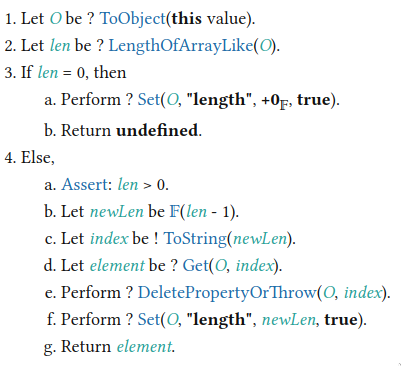
\includegraphics[width=0.6\textwidth]{images/array_pop.png}
    \caption{ECMAScript definition of Array.pop}
    \label{fig:Array_pop}
\end{figure}



% Internal Functions (LenghtOfArrayLike)
% printscreen do standard e explicacao
\paragraph*{LengthOfArrayLike internal function}
Figure \ref{fig:LengthOfArrayLike} shows a snippet of the ECMAScript standard description of the \texttt{LengthOfArrayLike} internal function, that evaluates the function:

\begin{center}
\texttt{LengthOfArrayLike (obj)}
\end{center}

\noindent The language starts by asserting that \texttt{obj} is an \texttt{Object} (step 1). Afterwards, gets the value of the property \texttt{length} from \texttt{obj} using the function \texttt{Get}. Then, converts the previously mentioned value to an Integer that represents the length with the \texttt{ToLength} function, and finally returns said Integer (step 2).

\begin{figure}[ht]
    \centering
    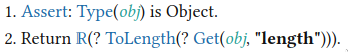
\includegraphics[width=0.5\textwidth]{images/length_array_like.png}
    \caption{ECMAScript definition of the LengthOfArrayLike}
    \label{fig:LengthOfArrayLike}
\end{figure}




\subsection{Test262}
\label{subsec:Test262}


% paragrafo - JS tem muitas particularidades que dificultam o desemvolvimento e testagem  -> É muito dificil desenvolver
% novas implemenentacoes da linguagem
% Existe uma bateria de testes que testa as implementacoes da
% linguagem contra o standard
% Esta bateria de testes é dificil de manter
% Porque? - muitos testes, muitas features, em geral ha retrocompatibilidade mas ha um pequeno numero de casos onde a retrocompatibilidade nao se verifica -> os testes de ser modificados
Implementing a \texttt{JavaScript} engine is particularly difficult since it involves dealing with the many corner cases that exist in the language. To test that corner cases are correctly dealt with there is \texttt{Test262}\cite{Test262}, the ECMAScript standard test battery. Although, \texttt{Test262} is vital to the \texttt{JavaScript} engines, it is very hard to maintain due it's complexity, the total number of tests is around \colorbox{orange}{39837} divided into \colorbox{orange}{87} subfolders, each correspond to roughly one section of the standard. \texttt{Test262} complexity grows with changes to the standard since in most cases backward compatible is maintained except for a few select cases. 
% 87 subfolders on built-ins + language
% QUESTION round number? (40000)
% QUESTION 105 subfolders if add intl402 (which also has files that were ignore)



% Implementacoes parciais da linguagem 
% Na acadamia é normal desenvolverem-se implementacoes parciais da linguagem: não suportam a ultima versao, não suportam todos os objectos built-in, não suportam todas
% Pergunta: Quais é que são os testes apropriados?
% Normal: Respostas ad-hoc -> sem justificação rigorosa -> basicamente cada paper selecciona os testes que lhe da jeito
Due to the ECMAScript standard being so extensive most implementations are only partial, especially implementations and analysis developed in academic contexts. In order to test partial implementations, one must be able to obtain the applicable set of tests from all the tests contained in Test262. Selecting the applicable tests is not a trivial matter because there are too many tests and too many features. The current methodology is that each development team manually selects the tests that are applicable to their corresponding implementation. This raises the problem that there is not standard and precise way of picking the all the right tests from the almost 40000 tests in \texttt{Test262}, making the possibility of human error when selecting the applicable tests likely.


% gosto
%% Formato dos testes
% frontmatter, code
% exemplo
Figure \ref{fig:Test262_example} shows a test from \texttt{Test262}. Every test of \texttt{Test262} has 3 parts: first is the copyright section represented with the comment \texttt{//} (lines 1 and 2), second is the \texttt{Frontmatter} section between \texttt{/*---} and \texttt{---*/} with some metadata about the test (lines 4 to 7), and finally is the \texttt{Body} section with the code of the test (lines 9 to 13). The copyright section has information about the owner and license of the test. The \texttt{Frontmatter} section has the test id (15.4.5-1) and a description of the test. Finally, the \texttt{Body}'s code tests the correct implementation of the standard.

\begin{figure}[ht]
    \centering
    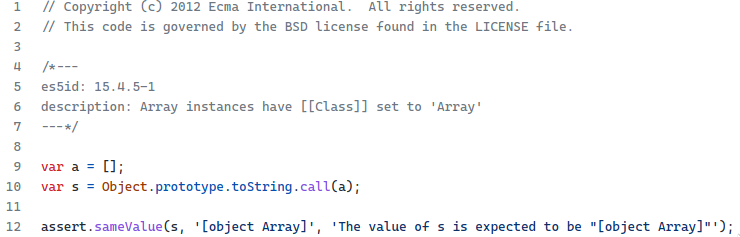
\includegraphics[width=1.0\textwidth]{images/test262_array_test.png}
    \caption{Test262 es5id: 15.4.5-1}
    \label{fig:Test262_example}
\end{figure}



%% metadados ja incluidos
%% referir outra vez o exemplo
% - metadados oficialmente incluídos nos testes
%   - que metadados é que os testes contém actualmente
The \texttt{Frontmatter} has keywords to hold metadata of the test. These keywords are associated with specific elements of metadata concerning the test. Bellow is the list of possible keywords and their meaning:

\begin{itemize}
\item \texttt{description} - contains a short description about what will be tested;
%
\item \texttt{esid} - contains the hash identifier of the ECMAScript portion associated with the feature that will be tested (the identifier references the most recent version of ECMAScript when the test is created);
%
\item \texttt{info} - contains a deeper explanation of the test behavior, frequently includes a direct citation of the standard;
%
\item \texttt{negative} - indicates that the test throws an error; associated to the keyword will be the type of error the test is supposed to be thrown (e.g. \texttt{TypeError}, \texttt{ReferenceError}) as well as the phase in which the error is expected to be thrown (e.g. \texttt{parse} vs \texttt{resolution} vs \texttt{runtime});
%
\item \texttt{includes} - contains the list of \texttt{harness} files that should be included in the execution of the tests (\texttt{Test262} makes use of a large number of auxiliary function defined in a dedicated library referred to as the \texttt{Test262} \texttt{harness} described later in this section);
%
\item \texttt{author} - contains the identification of the author of the test;
%
\item \texttt{flags} - contains a list of booleans for each test property, the properties being: (1) \texttt{onlyStrict}, the test is only executed in strict mode; (2) noStrict, the test will only be executed in mode \emph{sloppy}; (3) \texttt{module}, the test must be integrated as a \texttt{JavaScript} module; (4) \texttt{raw}, executes the test without any modification, which implies running as \texttt{noStrict}; (5) \texttt{async}, the test is contains asynchronous functions; (6) \texttt{generated}, the test generates the files specified by the property; (7) \texttt{CanBlockIsFalse} and (8) \texttt{CanBlockIsTrue}, the test will run if the property \texttt{CanBlock} of the \colorbox{orange}{\texttt{Agent Record}} executing it is false and true respectively; (9) \texttt{non-deterministic}, indicates that the semantics used in the test are intentionally under-specified and therefore the test passing or failing should not be regarded as an indication of reliability or conformance;
% QUESTION clarificar se e' necessario citar o que e' 'Agent Record' uma vez que nao vou explicar
%
%
\item \texttt{features} - contains a list of features that are used in the test;
%
\item \texttt{es5id} and \texttt{es6id} - indicates that the feature being tested belongs to ECMAScript 5 and 6 respectively and contains the hash identifier of the section of the standard it belongs to; these keywords have been deprecated and substituted by esid.
\end{itemize}


% Varias observacoes: 
%  - A metada esta muitas vezes INCOMPLETA e algumas vezes incorrecta 
%  - é preciso calcular a metadata certa
As Figure 5 illustrates, it is often the case that the metadata of a test is incomplete. Some tests also have the wrong metadata. As part of this thesis, we plan to process all the tests to check and correct their corresponding metadata as well as completing the metadata that is \colorbox{orange}{missing.}

%% QUESTION juntar os paragrafos?

%% metadados que achamos relevantes e nao estao incluidos
%% ...
\colorbox{orange}{The example} in Figure \ref{fig:Test262_example} has 2 keywords, description and the deprecated es5id. Besides the obvious upgrade from \texttt{es5id} to \texttt{esid} it would be useful to have \texttt{includes} with the \texttt{harness} files needed to execute the test. The \texttt{harness} information is very useful since it makes it easy to identify the part of the \texttt{harness} needed to run that test, opening the door for loading only part of the \texttt{harness} instead of the whole \texttt{harness} which is the current approach.



% - quais são os metadados que nós achamos serem relevantes e que estão em falta
\paragraph{New Metadata}
Besides the metadata that Test262 tests currently include, it would be useful for them to have additional information regarding:

\begin{itemize}
    \item \texttt{syntactic construct} - list of all syntactic constructions used in the test;
    \item \texttt{version} - the ECMAScript version of the standard in which the feature being tested was introduced;
    \item \texttt{built-ins} - list of all the built-ins used in the test.
    \item \texttt{harness-functions} - list of all the harness functions required to run the test.
\end{itemize}

This above metadata critical for filtering the tests when considering partial implementations of the language. For instance, if a JS engine only supports the 5th edition of the standard, one must be able to obtain all the corresponding tests for that \texttt{version}. Analogously, if a JS engine only implements certain \texttt{built-in} objects, one has to be able to filter out the tests that make use of the \texttt{built-in} objects that it does not implement. This would provide consistency and standardization to the selection of applicable tests to a partial implementation of the standard.
%
As for the \texttt{harness-functions}, it provides important information about the functions of \texttt{harness} that are used in the test. That information is relevant because only a small part of the \texttt{harness} is need in each test even though the whole library is loaded and tested. The harness has a total of 7290 lines in 32 files and is tested by 96 tests. By only including the exact functions that a test requires, one can speedup the testing process significantly.
% harness - has 32 files total 7290 lines (comments and blanck lines included)
% harness tests - has 96 files total 2646 lines (comments and blanck lines included)



\subsection{MetaData262 v0}
\label{subsec:MetaData262 v0}



% Para1 --> introduzir o trabalho do Miguel Trigo 
This thesis continues the master thesis of Miguel Trigo\cite{Thesis_Miguel_Trigo}, in which he developed a preliminary version of \texttt{MetaData262}. More specifically, he built a MongoDB database storing the metadata of all Test262 tests, representing the metadata of each test as a JSON object.



% Para2 --> estrutura da metadata
In \texttt{MetaData262 v0}, each test is associated with a JSON object storing the various metadata properties of the test and their corresponding values. Those metadata properties being the keywords of the \texttt{Frontmatter} mentioned in the previous section.
%
Besides, the existing metadata properties, various new properties were added to \texttt{MetaData262 v0}. We can divide these new properties into 3 main groups: location, extra front matter, and statistics. Each of these groups will be discussed next.

% Para 2.1 [path] (location)
\paragraph{Location group}
The location group contains information about the path to the test inside the \texttt{Test262}, having the property \texttt{path} associated to a string with the full path to the test.
% (ignored) there are also some properties that are subparts of the path and store their child.


% Para 2.2 [extra front matter: syntactic constructs, built-ins, version] 
\paragraph{Extra front matter group}
The extra front matter group contains new metadata generated for \texttt{MetaData262 v0}. The new metadata generated is associated with the properties: \texttt{syntactic\_construct}, \texttt{version}, and \texttt{builtIns} that were mentioned in the previous section as important metadata to add. \texttt{Version} stores the \texttt{ECMAScript} standard version the test belongs to. \texttt{Syntactic\_construct} stores an array with all the syntactic constructions that the test contains. As for \texttt{BuiltIns}, it stores all the built-ins that test interacts with and associates with each built-in its fields and functions that are used.


% Para 2.3 [statistics]
\paragraph{Statistics group}
Finally, the statistics group contains some statistical data about the tests. The properties this group has associated are \texttt{asserts}, \texttt{error}, \texttt{esprima}, and \texttt{lines}. The \texttt{asserts} property holds the amount of \texttt{assert} statements in the test. The \texttt{error} property stores the amount of calls made to the \texttt{Test262} error functions. The \texttt{esprima} property stores \emph{supported} or \emph{not supported} depending on whether \texttt{Esprima}\cite{Esprima} supports the test. \texttt{Esprima} is a standard-compliant \texttt{ECMAScript} parser that is also developed in \texttt{ECMAScript}, \texttt{Esprima} fully supports up to version 7 of the standard. The property \texttt{lines} holds the number of lines of code the test has, comments as well as empty lines are ignored.



% Para3 --> exemplo da MetaData262 v0 
Figure \ref{fig:json_metadata} shows the JSON object storing the metadata generated from the Test262 test given in Figure \ref{fig:Test262_example}. 
% Observacoes sobre o exemplo 
The JSON object begins with the \texttt{path} property and the path to the test associated with it. After, the \texttt{version} property indicates that this test belongs to the fifth version of the standard, if the version is not able to be calculated the field will be omitted. Followed by properties in the test's \texttt{Frontmatter} (note that the deprecated \texttt{es5id} is replaced to the \texttt{esid} property).
% ignorar as propriedades buit-ins e Array
Next is the \texttt{static\_construct} property that holds an array with the syntactic constructors of the test that were generated. The \texttt{builtIns} property holds a JSON object, in which, each property corresponds to a built-in and associated to it are its functions and fields that are interacted with in the test. Finally, the statistics group of properties. The \texttt{asserts} property that indicates that one assert statement is used in this test, the \texttt{error} holding zero since no error functions of the \texttt{Test262} were used in this test, the \texttt{esprima} property that indicates this test is supported by \texttt{Esprima}, and the \texttt{lines} property indicates that this test has 3 lines of code (the example in Figure \ref{fig:Test262_example} splits the last line of the test in order to improve the readability of the figure hence only 3 lines are counted in the actual test).


\begin{figure}[ht]
    \centering
    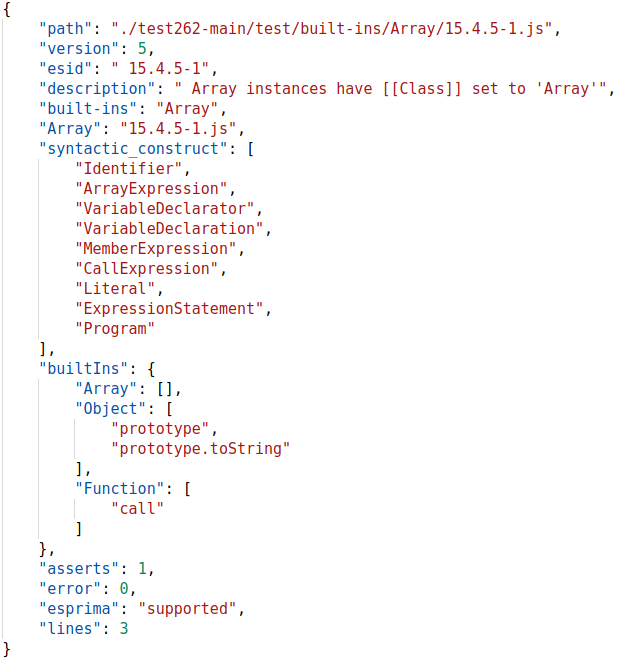
\includegraphics[width=0.9\textwidth]{images/json_metadata.png}
    \caption{Metadata generated for test esid: 15.4.5-1.js}
    \label{fig:json_metadata}
\end{figure}


% Para4 --> a metada original em falta teve de ser calculada e os 
% // bem como os novos campos da metadata -> 
As part of the setting up of MetaData262 v0,  M. Trigo had to compute the missing \texttt{Frontmatter} properties as well as the values of the new properties that he introduced. In most cases, the computation was straightforward, only involving a simple syntactic analysis of each test. However, the computation of the version and the built-ins used in each test was more involved and we will go through it in more detail below.
% [...]

% Para5 --> Version Computation 
\paragraph{Calculation of Version metadata}
The \texttt{version} of the standard a test belongs to is calculated using 3 different approaches: dynamic, static, and hybrid.
%
% dynamic approach
The dynamic approach is based on the waterfall model, running the tests in various JS engines, each corresponding to a specific version of the standard. As Figure \ref{fig:waterfall_model} illustrates, each test starts by running in the JS engine corresponding to version 5 of the \texttt{ECMAScript} standard (represented as ES). If the test output is correct then the test belongs to version 5 of the standard, otherwise the test will be run in the engine implementing the next version of the standard. This process repeats until the last engine, associated with version 11 of the standard, if the test output is not the expected again then the test is not supported.
%
% static approach
The static approach evaluates the syntactic tree of the test generated by \texttt{Esprima}, a widely used JS parser, as a JSON object. Starts by finding all the \texttt{JavaScript} keywords in the AST. Then associates each JS keyword with the version of the standard it was introduced in. Finally, the keyword with the most recent version associated will dictate the test version. For example, if the test has only two keywords associated with version 6 and 8, then the test will belong to the version 8 of the standard.
%
% hybrid approach
The hybrid approach is calculated using the results of the dynamic and static approaches. The hybrid approach merges the results by maintaining the higher version detected between each approach for each test. For instance, if the dynamic approach's result for a test is version 6 and the static's result for the same test is version 8, then, the test with belong to the version 8 of the standard according to the hybrid approach.



\begin{figure}[ht]
    \centering
    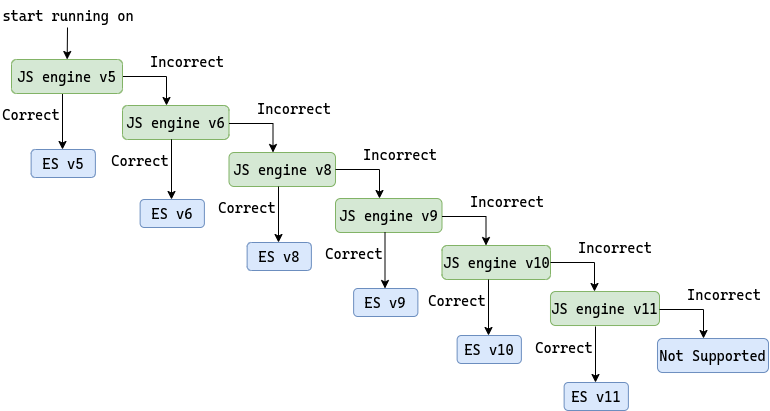
\includegraphics[width=1\textwidth]{images/waterfall_model.png}
    \caption{Waterfall model of the dynamic approach to calculate the ECMAScript version}
    \label{fig:waterfall_model}
\end{figure}




% Para6 --> Built-in Computation 
\paragraph{Calculation of built-ins metadata}
The \texttt{built-ins} used by each test are calculated using two separate approaches: dynamic and static. As in the calculation if the \texttt{ECMAScript} version both approaches are combined to improve the results. The static approach makes use of syntactic tree generated by \texttt{Esprima} as a JSON object from the test code. Next, traverses the AST to find expressions that interact with built-in objects. In addiction to the built-in, the fields and functions will also be outputted. As for the dynamic approach, it makes use of the built-ins functions in order to log whenever the function is called. In essence, a wrapper was created for each function that replaces it, the wrapper first logs that it was called, and then preforms the original method with the arguments that were supplied.




\section{Related Work}
\label{sec:Related Work}



\section{Design and Methodology}
\label{sec:Design and Methodology}



% Para1 --> problemas da metada existente na Metadata262 v0. 
% --> as versoes estao mal calculadas porque nao existem JS engines 
% que implementem exactamente uma versao e so essa versao 
% --> versoes calculadas em instalacoes ad-hoc 
% -- é preciso melhorar a analise dinamica considerando mais JS engines 
% --> os built-ins tb estao mal calculados porque a analise dinamica 
% dos built-ins ignora propriedades -> so considera chamadas a funcoes 
% por isso, se um teste for apenas: Array.prototype.pop = 3; 
% nao vai ser identificado como um teste que usa o array pela analise 
% dinamica 
% --> ha informacao em falta 
% ficheiros da harness e funcoes da harness
% Para 2 --> Problemas de acesso a metadata e obtencao de informacao estatistica 
% sobre os testes 
% --> neste momento quem quiser obter informacao estatisca sobre os 
% testes tem de interagir com uma base de dados Mongo e depois processar a informacao 
% como entender
% O objectivo desta tese é resolver estes dois problemas. 
% 5.1 - Precise Metadata for test262 tests 
% --> calcular a metadata precisamente 
% 5.1.1 versao -> 
% Montar um sistema escalavel para o calculo das versoes 
% associamos a cada versao um numero arbitrario de docker images cada uma 
% com um JS engine supostamente dessa versao 
% ---> parelelizacao etc
% 5.1.2 built-ins -> melhorar a instrumentcao para o calculo dinamico dos 
% built-ins --> em particular, apanhar property look-ups dinamicamente 
 
% 5.2 - MetaData Visualisation System 
% portal para visualizacao da metadata dos testes + informacao estatisca sobre os testes 
% --> gerar automaticamente 
% --> print screens do que ja fez
% --> discussao das bibliotecas que vai considera usar para criacao e display 
% da informacao estatisca 
% --> Exemplos de graficos a gerar 
% -- ...

% OLD DEPRECATED
\paragraph{OLD DEPRECATED} \colorbox{orange}{Para rescrever tudo com a nova estrutura!}


%  grandes objectivos 
This thesis is a continuation of Miguel Tringo's master thesis, aiming to complete the calculation of the \texttt{Frontmatter} metadata especially the \colorbox{orange}{metadata about the \texttt{harness}}, also aims to improve the generated metadata. Another aim of this thesis is to create a website for visualizing the metadata generated. \colorbox{orange}{Finally,} we aim to build a platform that allows users to submit the markdown generated from executing the \texttt{Test262} and compare different runs.
% QUESTION campo features? (restantes talvez possam ser ignorados author, negative, flags, info and description)
% QUESTION incluir?



% - processamento completo da metadata oficial 
% -> o processamento do miguel esta incompleto -> nao incluir informacao informacao sobre -> ... 
% [pode criticar como entender]
Miguel Trigo's thesis metadata is incomplete in various ways, tests with unknown \texttt{version} around 9000, tests without \texttt{built-ins} around 17000, and tests without \texttt{syntactic\_construct} around 13000 \colorbox{orange}{tests without esid around 600}.
% QUESTION sao tests da versao seginte de ECMA que ainda nao tem seccao na versao actual?
%
The metadata from the thesis could be improved in way the data is arranged, for example, the subfolders of the path to the test are spread into the JSON Object of the test. The subfolders information being put into an array of ordered subfolders would increase the readability.



% - calculo mais preciso da nova metadata proposta
% - o calculo da versao pode ser melhorado de varias maneiras
This thesis plans to improve the \texttt{version} metadata generation in two dimensions precision and efficiency.
% - Precisao 
% - usar mais engines
For the precision, with more \texttt{JavaScript} engines being used, there would be more certainty when determining the version.
% - Eficiencia 
% - paralelizar os engines 
As for the efficiency, it would be possible to parallelize the waterfall model of the dynamic approach running multiple tests at the same time. It is also possible to use \texttt{git diff} to identify the tests that were added or changed since the last time the dynamic approach was executed, \colorbox{orange}{ only needing to execute} the dynamic approach on the differences.
% QUESTION e' problema se fizerem update noutro lado que afeta o teste indiretamente?



% - Sistema de visualisacao da metadata 
The website for visualizing the metadata aims to make access to the metadata and filtering it easily accessible. The website is planned to allow the search 



% printscreens do site 
\begin{figure}[ht]
    \centering
    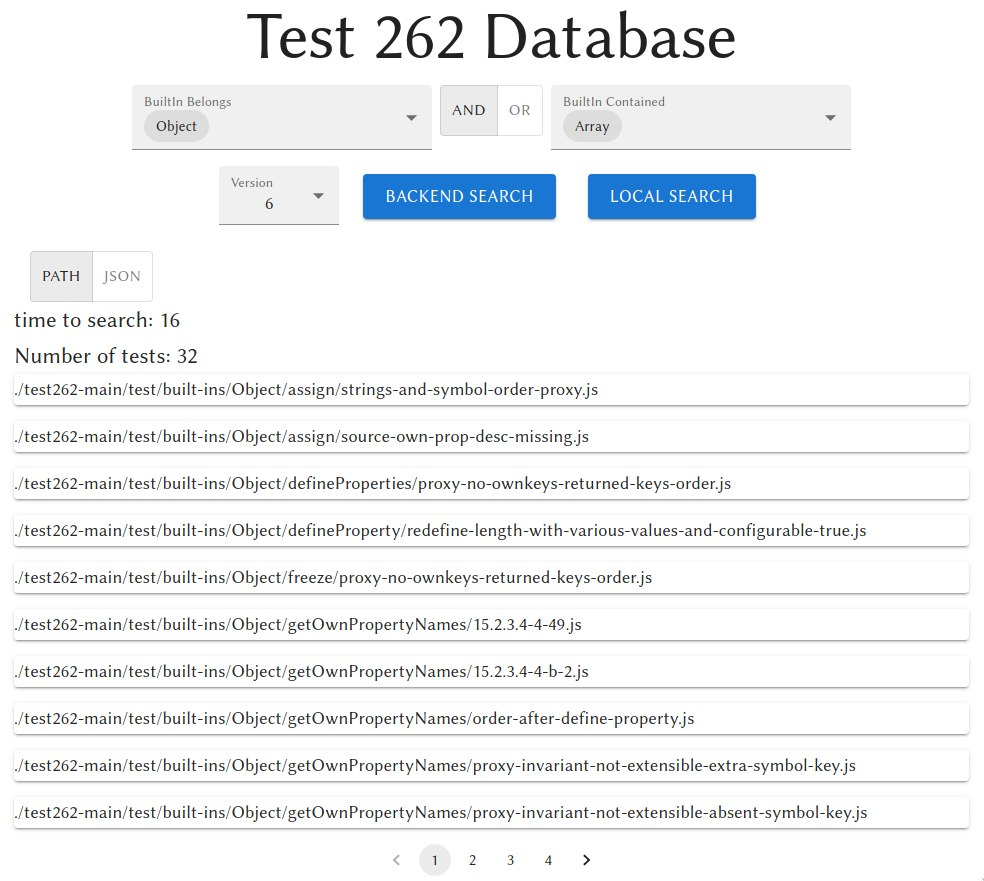
\includegraphics[width=1\textwidth]{images/website.png}
    \caption{Website for searching the metadata in construction}
    \label{fig:website}
\end{figure}

\section{Evaluation and Planning}
\label{sec:Evaluation and Planning}
% TODO GANT Diagram
\colorbox{orange}{pedir descricao da teses de uma das primeiras reunioes (iPad)}

\colorbox{orange}{Qual e' o plano pois nao tenho a certeza do que e' suposto realizar}

\section{Conclusion}
\label{sec:Conclusion}


%
% the environments 'definition', 'lemma', 'proposition', 'corollary',
% 'remark', and 'example' are defined in the LLNCS documentclass as well.
%

%
% ---- Bibliography ----
%
% BibTeX users should specify bibliography style 'splncs04'.
% References will then be sorted and formatted in the correct style.
%
% \bibliographystyle{splncs04}
% \bibliography{mybibliography}
%
\bibliographystyle{splncs04}
\bibliography{references}

\end{document}
